\subsection{Connecting the Dots: Understanding Load and Line Interaction!}

\begin{tcolorbox}[colback=gray!10, colframe=black, title=E9E07] What parameter describes the interaction of a load and transmission line?
\begin{enumerate}[label=\Alph*)]
    \item A: Characteristic impedance
    \item \textbf{B: Reflection coefficient}
    \item C: Velocity factor
    \item D: Dielectric constant
\end{enumerate} \end{tcolorbox}

\subsubsection{Concepts Related to Load and Transmission Line Interaction}

To understand the interaction between a load and a transmission line, we need to grasp several key concepts in radio communication and electronics. 

1. \textbf{Transmission Line:}: This is a specialized cable or other structure that serves to conduct electromagnetic waves in a controlled manner, typically used to connect components of an RF communication system.

2. \textbf{Load:}: This refers to any component that consumes power from the transmission line. Common examples include antennas, resistors, or other circuit elements.

3. \textbf{Reflection Coefficient:}: The reflection coefficient is a critical parameter that quantifies how much of the electromagnetic wave is reflected back towards the source when it encounters a load. The reflection coefficient (\( \Gamma \)) is defined as:
   \[
   \Gamma = \frac{Z_L - Z_0}{Z_L + Z_0}
   \]
   where \( Z_L \) is the impedance of the load and \( Z_0 \) is the characteristic impedance of the transmission line. 

4. \textbf{Characteristic Impedance:}: This is the impedance that a transmission line would present if it were infinitely long. It is determined by the physical and material properties of the line.

5. \textbf{Velocity Factor:}: This is the ratio of the speed of a signal through a transmission line compared to the speed of light in a vacuum.

6. \textbf{Dielectric Constant:}: This is a measure of a material's ability to store electrical energy in an electric field and affects the speed and impedance of the signal.

\subsubsection{Calculation Example}

To illustrate the concept, let's say we have a transmission line with a characteristic impedance \( Z_0 = 50 \, \Omega \) and a load with an impedance \( Z_L = 75 \, \Omega \). We can calculate the reflection coefficient as follows:

\[
\Gamma = \frac{Z_L - Z_0}{Z_L + Z_0} = \frac{75 - 50}{75 + 50} = \frac{25}{125} = 0.2
\]

A reflection coefficient of 0.2 indicates that 20\% of the signal is reflected back towards the source when it reaches the load.

\subsubsection{Visual Representation}

Below is a simple diagram using TikZ that illustrates the reflection of a wave at the load.

\begin{center}
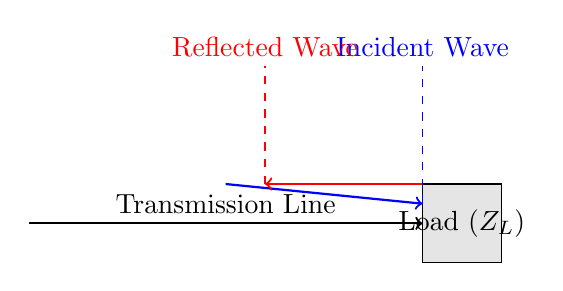
\begin{tikzpicture}
    % Draw the transmission line
    \draw[->, thick] (0,0) -- (5,0) node[midway, above] {Transmission Line};

    % Draw the load
    \draw[draw=black, fill=gray!20] (5,-0.5) rectangle (6,0.5) node[midway] {Load ($Z_L$)};
    
    % Representing the incident wave
    \draw[->, blue, thick] (2.5, 0.5) -- (5,0.25);
    \draw[dashed, blue] (5,0.25) -- (5,2) node[above] {Incident Wave};

    % Representing the reflected wave
    \draw[->, red, thick] (5,0.5) -- (3,0.5);
    \draw[dashed, red] (3,0.5) -- (3,2) node[above] {Reflected Wave};
\end{tikzpicture}
\end{center}

Through this understanding of the reflection coefficient and the related parameters, we can draw insights on how a load interacts with a transmission line in practical scenarios.
